\documentclass[letterpaper]{article}
\usepackage{natbib,alifeconf}

\title{Report on the Neural Network Training for the project: Assessing Economic Development and Planning Interventions in the Built Environment: The Role of Provincial Policies in Québec and Ontario}
\author{Alphonsus Adu-Bredu$^{1}$ \\
\mbox{}\\
$^1$Tufts University, Medford - Massachusetts \\
alphonsus.adu\_bredu@tufts.edu}


\begin{document}
\maketitle

\begin{abstract}
	The dataset was first split into the 6 categories; "depressing", "lively", "safety", "wealthy", "boring" and "beauty". All the operations reported in this paper were made to the depressing category.
\end{abstract}
\section{Data Preprocessing}
After the categorization, the dataset was cleaned up by removing all datapoints that appeared in both the positive and negative sub-categories. The coordinates for all positive datapoints(images that are depressing) were retrieved. 

\section{Neural network Analogy}
Training a neural network model can be compared to studying for an exam using a set of practice problems. When we train the neural network, we get the model to study the entire set of practice problems and their corresponding solutions(training dataset) for a number of times (number of iterations). Then we get the model to take the actual exam (cross-validation). The model's performance in studying the practice problems is indicated by a measure called the training accuracy. And it's performance in the actual exam is indicated in the cross-validation accuracy.\\
In the experiments below, I tune the hyperparameters, thus, the number of iterations and the quantity of training data in order to get an optimum training and cross-validation accuracy.\\

\section{Downloading images and training neural network}
For the first batch of training, the first 250 coordinates of both the positive datapoints and their corresponding negative datapoints were retrieved and their corresponding street-view images were downloaded. After the images were downloaded, a convolutional neural network was trained on the positive and negative images. 

In training the convolutional neural network, a method called Transfer Learning was employed. We first downloaded Google's pre-trained inception-v3 model and retrained the last two layers in the network with our 250 depressing images and 250 non-depressing images to get it to classify images into those two categories. The training process was first ran for 500 iterations. A graph of the training accuracy over the 500 iterations is in Figure 1.

\begin{figure}[!htb]
	\begin{center}
		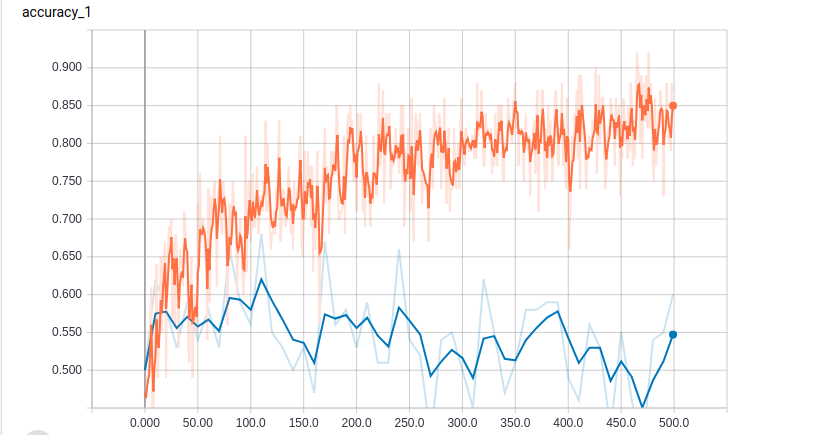
\includegraphics[width=4in]{250_img_500_it_accuracy.png}
		\caption{250 images, 500 iterations. Training accuracy = Red, Cross-validation accuracy=Blue}
		\label{fig1}
	\end{center}
\end{figure}

The average training accuracy was around 85\% while the cross-validation accuracy lingered around 50\%.

The number of iterations was increased to 2500 and the training accuracy rose to 98\% while the cross-validation accuracy still lingered around 50\%. [Figure 2]This meant that our trained model was over-fitting on the training set. A common remedy for this would be to increase the number of training images.\\


\begin{figure}[!htb]
	\begin{center}
		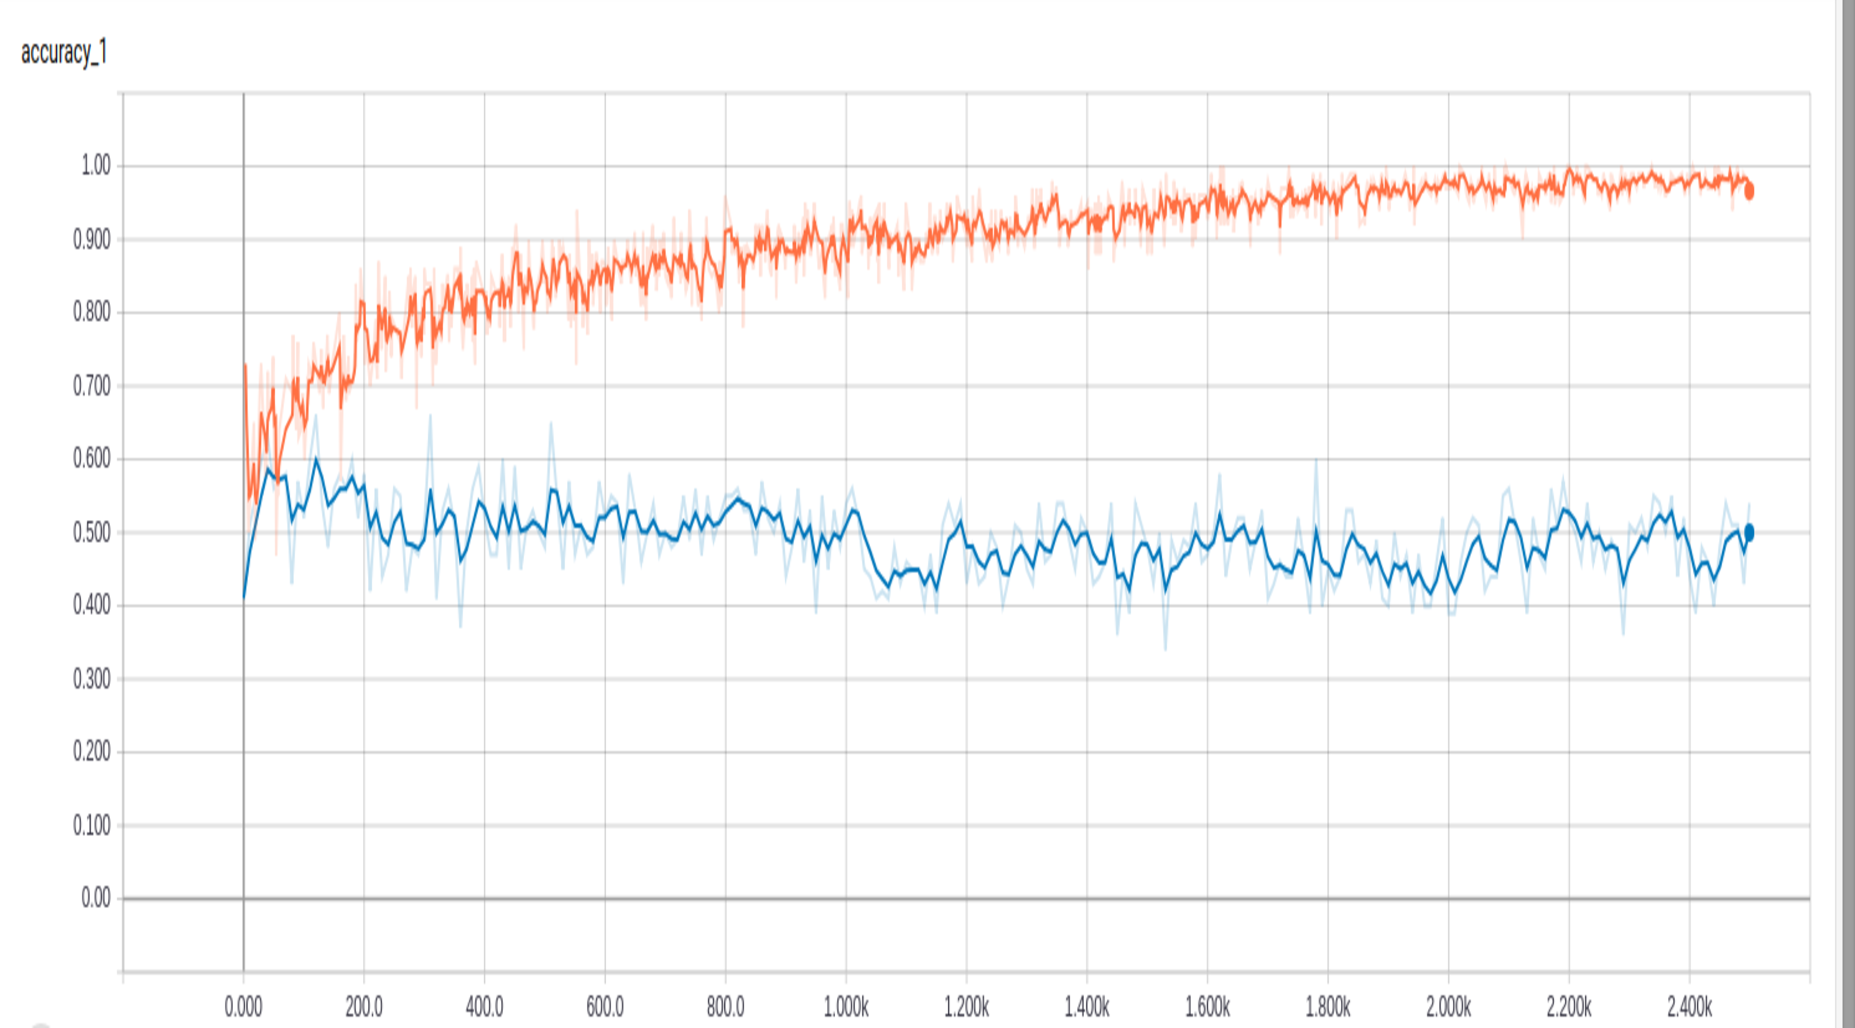
\includegraphics[width=3.5in]{250_img_2500_it_accuracy.png}
		\caption{250 images, 2500 iterations. Training accuracy = Red, Cross-validation accuracy=Blue}
		\label{fig2}
	\end{center}
\end{figure}

The dataset was then increased by 484 images. Resulting in a total of 734 images for the positive 'depressing' category and 734 images for the negative  'depressing' category. The neural net was retrained with these new set of images for 2500 iterations. It had an average 82\% training accuracy and 50\% cross-validation accuracy [Figure 3]. 

\begin{figure}[!htb]
	\begin{center}
		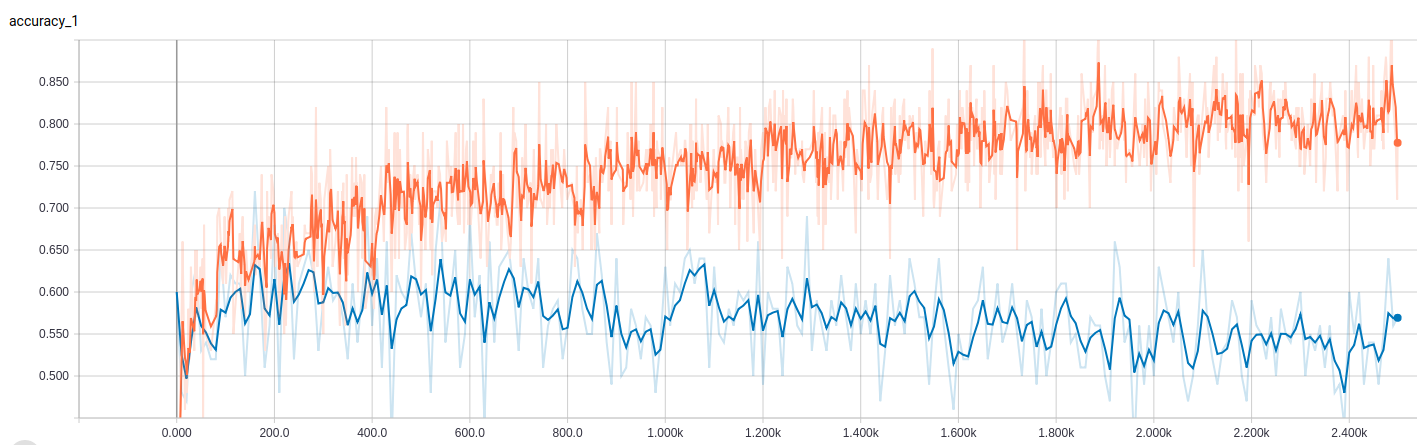
\includegraphics[width=3.5in, height=2.5in]{734_img_2500_it_accuracy.png}
		\caption{734 images, 2500 iterations. Training accuracy = Red, Cross-validation accuracy=Blue}
		\label{fig3}
	\end{center}
\end{figure}

%\vspace*{0.1in}
\newpage
The number of iterations was then increased to 5000. The training accuracy rose to 94\% and the cross-validation accuracy still lingered at 56\%[Figure 4].It seemed that the cross-validation accuracy wouldn't improve substantially with any more increase in the number of iterations. 

\begin{figure}[!htb]
	\begin{center}
		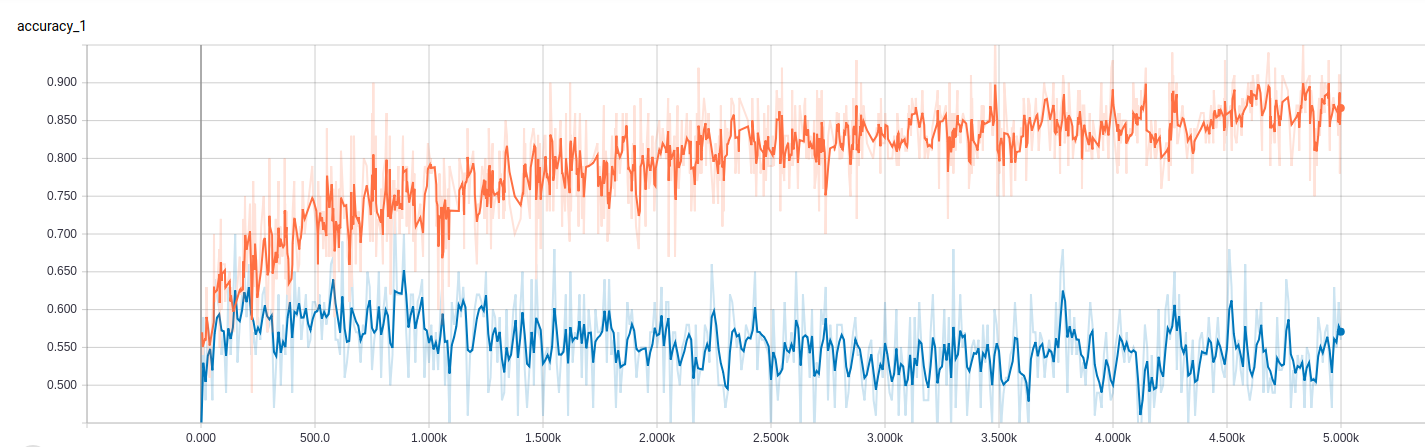
\includegraphics[width=3.5in, height=2.5in]{734_img_5000_it_accuracy.png}
		\caption{734 images, 5000 iterations. Training accuracy = Red, Cross-validation accuracy=Blue}
		\label{fig1}
	\end{center}
\end{figure}


%\vspace*{2.5in}
\section{Reflections}
Considering how the cross-validation accuracy varied only slightly even after the numerous alterations of the structure of our data and the neural network, it seems unlikely that it would improve drastically if the quantity of the dataset is increased any further. A probable cause for the inability of the trained model to distinguish between the two categories could be our ground-truth data, the manner in which our data was labeled. The original labeling was done relatively, thus, two images were compared and one was chosen to be more depressing than the other. Even though this didn't necessarily mean the less-depressing image was exactly not depressing, we made the conscious decision to label the less-depressing image as not-depressing. This, as a result, could have made it more difficult for the neural network to learn a general difference between depressing and not-depressing images. 




%\begin{table}[!hbt]
%\center{
%\begin{tabular}{|c|c|c|}\hline
%One & Two & Three\\ \hline\hline
%Yes & 0 & 1 \\
%Not  & 1 & 0 \\
%Maybe & 0.5 & 0.5 \\ \hline
%\end{tabular}
%}
%\vskip 0.25cm
%\caption{Sample table caption.}
%\end{table}


%\footnotesize
%\bibliographystyle{apalike}
%\bibliography{sample}


\end{document}
